\subsection{REDUCTIVE LIE ALGEBRAS}

DEFINITION 4. A Lie algebra is called reductive if its adjoint representation is semi-simple.

PROPOSITION 5. Let \(\mathfrak{g}\) be a Lie algebra and \(\mathfrak{r}\) its radical. The following conditions are equivalent:

\begin{enumerate}
\def\labelenumi{(\alph{enumi})}
\item
  g is reductive.
\item
  \(\mathcal{D}\mathfrak{g}\) is semi-simple.
\item
  \(\mathfrak{g}\) is the product of a semi-simple algebra and a commutative algebra.
\item
  \(\mathfrak{g}\) has a finite-dimensional representation such that the associated bilinear form is non-degenerate.
\item
  \(\mathfrak{g}\) has a faithful semi-simple finite-dimensional representation.
\item
  The nilpotent radical of g is zero.
\item
  r is the centre of g.
\item
  \(\Rightarrow\) (b): if the adjoint representation of \(\mathfrak{g}\) is semi-simple, \(\mathfrak{g}\) is a direct sum of minimal non-zero ideals \(a_{i}\) and hence \(\mathfrak{g}\) is isomorphic to the product of the \(a_{i}\) ; and \(a_{i}\) has no ideals other than \(\{0\}\) and \(a_{i}\) and hence is simple or commutative of dimension 1. Therefore \(\mathcal{D}\mathfrak{g}\) is equal to the product of those \(a_{i}\) which are simple and hence is semi-simple.
\item
  \(\Rightarrow\) (c): if \(\mathcal{D}\mathfrak{g}\) is semi-simple, \(\mathfrak{g}\) is isomorphic to the product of \(\mathcal{D}\mathfrak{g}\) by a Lie algebra \(\mathfrak{h}\) (no. 1, Corollary 1 to Proposition 1); \(\mathfrak{h}\) is isomorphic to \(\mathfrak{g}/\mathcal{D}\mathfrak{g}\) and hence is commutative.
\item
  \(\Rightarrow\) (d): let \(g_{1}\) and \(g_{2}\) be two Lie algebras, \(\rho_{i}\) a finite-dimensional representation of \(g_{i}\) and \(\beta_{i}\) the bilinear form on \(g_{i}\) associated with \(\rho_{i}\) (i = 1, 2); \(\rho_{1}\) and \(\rho_{2}\) can be considered as representations of \(g = g_{1} \times g_{2}\) ; let \(\rho\) be their direct sum. Clearly the bilinear form on g associated with \(\rho\) is the direct sum of \(\beta_{1}\) and \(\beta_{2}\) and hence is non-degenerate if \(\beta_{1}\) and \(\beta_{2}\) are non-degenerate. Then to prove the implication (c) \(\Rightarrow\) (d) it suffices to consider the 2 following cases: (1) g is semi-simple; then the adjoint representation admits as associated form the Killing form, which is non-degenerate; (2) g = K; then the identity representation of g on K has an associated bilinear form which is non-degenerate.
\end{enumerate}

\((d) \Rightarrow (e)\) : let \(\rho\) be a finite-dimensional representation of \(g\) and \(\beta\) the associated bilinear form; by Proposition 4 of §4, no. 3, there exists a finite-dimensional semi-simple representation \(\sigma\) of \(g\) such that the kernel \(n\) of \(\sigma\) is orthogonal to \(g\) with respect to \(\beta\) . If \(\beta\) is non-degenerate, then \(n = \{0\}\) and hence \(\sigma\) is faithful.

\begin{enumerate}
\def\labelenumi{(\alph{enumi})}
\setcounter{enumi}{4}
\tightlist
\item
  \(\Rightarrow\) (f): this is obvious.
\end{enumerate}

\((f) \Rightarrow (g)\) : if the nilpotent radical of \(g\) is zero, \(\mathcal{D}g \cap r\) is zero ( \(\S 5\) , no. 3, Theorem 1); as \([g, r] \subset \mathcal{D}g \cap r\) , \(r\) is the centre of \(g\) .

\begin{enumerate}
\def\labelenumi{(\alph{enumi})}
\setcounter{enumi}{6}
\tightlist
\item
  \(\Rightarrow\) (a): if \(\mathfrak{r}\) is the centre of \(\mathfrak{g}\) , the adjoint representation of \(\mathfrak{g}\) is identified with a representation of \(\mathfrak{g} / \mathfrak{r}\) , which is a semi-simple Lie algebra (§ 5, no. 2, Proposition 3); this representation is therefore semi-simple (Theorem 2).
\end{enumerate}

Remark. If a Lie algebra g can be decomposed as a product \(a \times b\) of a commutative Lie algebra a and a semi-simple Lie algebra b, this decomposition is unique. More precisely, the centre of g is equal to the product of the centres of a and b and is hence equal to a. And \(\mathcal{D}g = \mathcal{D}a \times \mathcal{D}b = b\) .

COROLLARY. (a) Every finite product of reductive algebras is a reductive algebra.

\begin{enumerate}
\def\labelenumi{(\alph{enumi})}
\setcounter{enumi}{1}
\item
  If \(\mathfrak{g}\) is a reductive Lie algebra of centre \(\mathfrak{c}\) , every ideal of \(\mathfrak{g}\) is a direct factor, the product of its intersections with \(\mathfrak{c}\) and \(\mathcal{D}\mathfrak{g}\) , and is a reductive Lie algebra.
\item
  Every quotient of a reductive Lie algebra is a reductive Lie algebra.
\end{enumerate}

Assertion (a) follows for example from condition (c) of Proposition 5.

Suppose that g is reductive. Let a be an ideal of g. Since the adjoint representation of g is semi-simple, a has a supplementary ideal b and g is identified with \(a \times b\) . For all \(x \in g\) , let \(\rho(x)\) be the restriction of \(ad_{g}x\) to a. Then \(\rho\) is a semi-simple representation of g which is zero on b and defines on passing to the quotient the adjoint representation on a. Hence a is reductive. Similarly, g/a and b, which are isomorphic, are reductive. Finally, let \(b, b'\) be the centres of a and b; then \(a = b \times Da\) , \(b = b' \times Db\) , \(b \times b' = c\) , \(Da \times Db = Dg\) ; hence \(a = (a \cap c) + (a \cap Dg)\) .

PROPOSITION 6. Let g be a Lie algebra, r its radical and s its nilpotent radical.

\begin{enumerate}
\def\labelenumi{(\alph{enumi})}
\item
  \(\mathfrak{s} = [\mathfrak{g},\mathfrak{r}] = \mathcal{D}\mathfrak{g}\cap \mathfrak{r}.\)
\item
  s is the intersection of the orthogonals of g with respect to the bilinear forms associated with the finite-dimensional representations of g.
\end{enumerate}

Clearly \([\mathfrak{g},\mathfrak{r}]\subset \mathcal{D}\mathfrak{g}\cap \mathfrak{r}\) . Now \(\mathcal{D}\mathfrak{g}\cap \mathfrak{r} = \mathfrak{s}\) by Theorem 1 of §5, no. 3. Let \(\mathfrak{g}' = \mathfrak{g}/[\mathfrak{g},\mathfrak{r}]\) and \(f\) be the canonical homomorphism of \(\mathfrak{g}\) onto \(\mathfrak{g}'\) ; then \(f(\mathfrak{r})\) is the radical \(r'\) of \(\mathfrak{g}'\) (Corollary 3 to Proposition 2, no. 2), hence \([\mathfrak{g}',\mathfrak{r}'] = \{0\}\) and \(r'\) is the centre of \(\mathfrak{g}'\) ; therefore (Proposition 5) \(\mathfrak{g}'\) has a finite-dimensional faithful semi-simple representation, whence \(\mathfrak{s}\subset [\mathfrak{g},\mathfrak{r}]\) . This proves (a).

Let \(t\) be the intersection of the orthogonals of \(\mathfrak{g}\) with respect to the bilinear forms associated with the finite-dimensional representations of \(\mathfrak{g}\) . Then \(\mathfrak{s} \subset t\) ( \(\S 4\) , no. 3, Proposition 4 (d)). On the other hand, \(\mathfrak{g}/\mathfrak{s}\) has a finite-dimensional faithful semi-simple representation and hence (Proposition 5) a finite-dimensional representation \(\rho\) such that the associated bilinear form is non-degenerate; considered as a representation of \(\mathfrak{g}\) , \(\rho\) has an associated bilinear form \(\beta\) on \(\mathfrak{g}\) and the orthogonal of \(\mathfrak{g}\) with respect to \(\beta\) is \(\mathfrak{s}\) , whence \(t \subset \mathfrak{s}\) . Hence \(t = \mathfrak{s}\) .

\pandocbounded{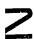
\includegraphics[keepaspectratio]{images/part001_ead1ec0a.jpg}}

Even if \(s \neq \{0\}\) there may exist non-degenerate symmetric bilinear forms on g (Exercise 18 (c)). Such forms, of course, are not associated with any representation of g.

COROLLARY. Let \(\mathfrak{g},\mathfrak{g}'\) be Lie algebras, \(\mathfrak{s}\) (resp. \(\mathfrak{s}'\) ) the nilpotent radical of \(\mathfrak{g}\) (resp. \(\mathfrak{g}'\) ) and \(f\) a homomorphism of \(\mathfrak{g}\) onto \(\mathfrak{g}'\) .

\begin{enumerate}
\def\labelenumi{(\alph{enumi})}
\item
  Then \(\mathfrak{s}' = f(\mathfrak{s})\) .
\item
  \(\mathfrak{g}'\) is reductive if and only if the kernel of \(f\) contains \(\mathfrak{s}\) .
\end{enumerate}

If \(\mathfrak{r},\mathfrak{r}'\) are the radicals of \(\mathfrak{g},\mathfrak{g}',\) then \(\mathfrak{s}' = [\mathfrak{g}',\mathfrak{r}'] = [f(\mathfrak{g}),f(\mathfrak{r})] = f([ \mathfrak{g},\mathfrak{r}]) = f(\mathfrak{s})\) . Assertion (b) is an immediate consequence of (a).

